%%%%%%%%%%%%%%%%%%%%%%%%%%%%%%%
%%% 第一章 绪论
%%%%%%%%%%%%%%%%%%%%%%%%%%%%%%%
\chapter{绪论}

%%% 1.1 论文研究背景及意义
%%%%%%%%%%%%%%%%%%%%%%%%%%%%%%% 
\section{论文研究背景及意义}
\subsection{研究背景}

人工智能的迅速发展将深刻改变人类社会生活,改变世界。为此,国务院在2017年7月8日向
各省、自治区、直辖市人民政府等印发了《新一代人工智能发展规划》     \cite{GWY:2017}。
此规划是为了推动人工智能
快速发展,造福民生。其中,“人工智能+”是其中的重要环节。所谓“人工智能+”,就是将人工智能与各个传统行业深度融合,
深入改造各个传统行业,帮助传统行业转型,创造新的产业形态。而智能制造则是人工智能与制造业的深度融合。十八大以来,
“制造业转型升级”等战略被逐步提出,但对于中国制造来说,要实现转型升级,首先要考虑由劳动密集型向技术密集型转变。而
人工智能技术与制造业的融合可以代替大量劳动力,实现工业自动化,助力“中国制造2025”,帮助中国制造转型升级。

工业机器人,按照ISO 8373    \cite{ISO:1994}
的定义,是面向工业领域的多关节机械手或多自由度的机器人。工业机器人通过预先编写
的程序可以实现重复性动作,以此可来代替一些重复性的人工工作,是制造业中非常重要的劳动力代替工具。根据国际机器人联合会发布的
2012年世界机器人研究报告,在2011年年底,世界上运行中的工业机器人数量达1153000。可以说,工业机器人的每次技术进步,都能带来
制造业工作效率质的提升。

分拣作业是制造业中非常常见的一种作业场景,由于其重复性强、作业场景单一的任务特性,分拣作业成为工业机器人的重要应用场景之一。
传统的工业分拣采用人工方法,不但耗时耗力,而且无法满足自动化长时间作业,影响生产效率的提升。而传统的工业机器人自动分拣系统,
采用预先编程的工业机器人进行工业分拣,虽然能够实现重复性动作的复现,但由于工业机器人无法根据实际情况改变自身动作,所以这种系统
对分拣件的摆放位置有严格的设定,且该系统只能进行分拣,无法进行分类。因此,近年来,越来越多的学者将机器视觉应用到工业机器人当中,
使机器人具备人眼功能,能够根据工件位置自适应地调整机器人动作,并且能够实现分拣和分类。基于机器视觉的工业机器人系统具备更好的鲁棒性,
因此越来越多的机器视觉工业机器人投入到实际应用中,不仅提高了生产产品质量,更保证了工业化生产的效率  \cite{CJF:2011}。

机器视觉技术是利用机器代替人眼做各种测量和判断的技术    \cite{BZG:2015}。
工业自动分拣系统主要由机器人、视觉传感装置、
图像采集装置和图像处理系统构成  \cite{ZWH:2018},
其中机器人模块主要执行图像处理系统所返回的指令,其他模块构成了机器视觉模块,
负责获取所需识别物体的位置及类别。由于机器人模块受环境影响较小,而图像处理模块需要满足工业环境中的实时性和快速性要求,而且需要对
工厂复杂多变的环境有较高的适应性。因此,机器视觉中的目标检测算法是整个视觉自动分拣系统中的核心。

人工智能的高速发展必定伴随着对各行各业的改造。以深度学习为代表的算法也在不断颠覆各种传统机器视觉算法。将深度学习应用到基于视觉的工业分拣
系统中,不仅能够提高视觉识别的效果,而且得益于深度学习的端到端的特性,系统的可移植性也可以得到提高。本文研发的基于深度学习的机械臂分拣系统
及其云平台,将深度学习应用到自动分拣系统的核心模块:目标检测,并且研发出一套基于深度学习,用于训练目标检测算法的云平台,降低视觉应用门槛,
具备更强的通用性。

\subsection{研究意义}

随着“中国制造2025”的提出,中国正迈向“制造大国”到“制造强国”的道路。中国制造业自动化转型迫在眉睫。工业机器人,作为
制造业中不可或缺的生产工具,在制造业自动化中扮演着重要角色。工业机器人任何技术上的提升必定带来制造业生产效率的提升。
因此,对工业机器人的技术研究对实现“中国制造2025”具有重要意义。

作为工业机器人应用的重点和难点,工业分拣系统具备大多数工业机器人的技术应用场景。工业自动分拣系统的研究突破势必带动工业机器人
技术的进步。工业自动分拣系统主要包括图像采集模块、图像处理模块、机器人模块。其中,图像采集模块主要用于获取分拣件图像信息,作为图像处理
模块的输入;图像处理模块主要根据图像采集模块采集得到的图像信息,进行计算,得到分拣件位置和类别信息,并将该信息发送给机器人模块执行;机器人模块
根据分拣件位置和类别信息,对分拣件进行抓取并放到合适位置。这其中,图像处理模块是整个系统的中枢,决定了整个系统的实时性和准确性。一个好的图像
处理模块带来的系统性能提升是其他模块无法比拟的。

分拣系统中用到的图像处理算法主要为目标检测算法。目标检测算法可以根据是否应用深度学习技术,将之分为传统目标检测算法和基于深度学习的目标检测算法。
传统的目标检测算法需要人为构造特征,且针对不同检测物体需要构造相应的特征。当需要检测的物体数量变多并且经常发生变化时,传统的目标检测方法就会显得
捉襟见肘。而基于深度学习的目标检测算法可以实现端到端的训练和预测。同时,深度学习端到端的特性既方便了模型的训练,又方便模型的移植。针对不同的检测
场景,只需要标注相应数量的数据,利用迁移学习    \cite{TransferL:2010}
技术,在ImageNet  \cite{ImageNet:2009}
的预训练参数上进行fine-tune,即可得到良好的可用模型。

鉴于以上特性,根据当前工业自动分拣系统及我国制造业特性,提出了本论文的基本设想,即开发一套基于深度学习的机械臂分拣系统,同时将深度学习模型的训练过程
开放到云平台。本论文的设想分两部分:一是将基于深度学习的目标检测算法应用到工业分拣系统当中,验证其可行性及效果;二是开发基于深度学习的目标检测模型训练
云平台,帮助制造业从业者生成他们所需的目标检测模型。相对应地,本论文有如下两部分意义:一是研究深度学习在工业分拣系统中的应用效果,提高工业自动分拣系统的
分拣质量及鲁棒性;二是从我国制造业从业者深度学习知识普及度不高的事实出发,将深度学习模型的训练过程封装为对制造业从业者友好的网页界面,从而普及深度学习在工业
自动分拣系统甚至是整个制造业中的应用。

%\begin{figure}
%\centering
%\includegraphics{}
%\caption{}
%\label{Figflag} 
%\end{figure}

%%% 1.2 国内外研究现状
%%%%%%%%%%%%%%%%%%%%%%%%%%%%%%
\section{国内外研究现状}
%%% 1.2.1 目标检测算法研究现状
%%%%%%%%%%%%%%%%%%%%%%%%%%%%%%
\subsection{目标检测算法研究现状}
目标检测是机器视觉中的一个重要问题,在轨迹跟踪、自动驾驶、工业分拣等生活及工业领域都具有重要的应用和研究价值。早期的目标检测算法
主要是人工构造特征,通过模板和传统机器学习方法进行检测。然而,2012年,Hinton等人提出了AlexNet   \cite{NIPS2012_4824},
在ImageNet
的表现超出第二名41\%,将深度学习的革命性效果带到大众眼前。深度学习在图像分类任务上的良好表现,促使各界学者纷纷在各自的领域应用深度学习,
由此催生出一批基于深度学习的优秀算法。目标检测任务也不例外。

自目标检测的概念提出以来,国内外学者针对目标检测算法进行了一系列探索。在深度学习兴起之前,传统的目标检测算法大致分为目标实例检测和传统
目标类别检测两类    \cite{MBJC:2018}:
\begin{enumerate}
    \item{目标实例检测,即通过模板和人工提取的特征点,获得模板与检测对象的对应关系,检测出目标对象。}
    \item{目标类别检测则通过使用传统的机器学习方法,根据人工提取的特征和选定的分类器,检测出实现定义好的有限几种类别。}
\end{enumerate}

2004年,Lowe等提出在目标实例检测方面应用极为广泛的SIFT  \cite{Lowe2004}
算法,该算法使用高斯模糊来实现尺度空间,使用高斯差分函数
进行极值检测,再通过对各个因素的判定和筛选,得出匹配度高、抗噪性强的关键点。但该算法存在复杂度高、速度慢、对于特征不明显图像很难提取特征
点等问题。针对这些问题,Ke等人同年提出了PCA-SIFT    \cite{PCA-SIFT:2004}
算法。该算法引入PCA方法对SIFT算法中的向量进行降维,以提高匹配效率。但
由于降维损失了部分信息,因此该算法虽然提高了匹配效率,但匹配效果具有局限性。同样基于SIFT,2006年提出的SURF  \cite{SURF2006}
算法则引入了Hessian
矩阵,减小了计算量,提高了目标检测的速度。而目标类别检测方面,使用较多的则是基于AdaBoost    \cite{AdaBoost1996}
的系列算法。AdaBoost算法是一种Boosting算法,能够将多个弱学习器,通过调整训练集样本权重的方法,组合为一个强学习器。

传统的目标检测算法,其目的都是在人工提取丰富特征点的前提下,尽可能减少计算量,从而提高计算效率,提高识别速度。但人工提取特征虽然易于理解,
简单直观,但无法应对大量类别的识别,在目标识别体发生变化时,需要针对性地再次进行繁杂的特征设计和提取工作。而基于深度学习的目标检测算法,使用神经
网络提取图像底层和高层特征,不仅能够提取出更加丰富、表达性更强的特征,而且不需要人工参与特征的提取,还能做到端到端的训练和预测。

基于深度学习的目标检测算法分为两类。一类是基于分类的目标检测算法(two-stage),另一类则是以回归的方式来进行目标检测的算法(single-stage)。
顾名思义,two-stage的方法,采用两步来进行目标检测:1. 生成可能区域(Region Proposal)并且使用CNN提取特征。2. 使用分类器分类并修正位置。这类方法
的代表是R-CNN   \cite{RCNN:2014}。
2014年,Ross等人提出了R-CNN。该算法使用Selective Search获得候选区域,然后进行归一化,作为CNN网络的输入。再使用神经网络获取候选区域的特征,最后利用
多个SVM分类器进行分类。R-CNN大幅度提高了目标检测的准确率,但由于R-CNN是对所有的候选区域进行特征提取和计算,多个候选区域之间的重叠区域重复计算了多次,导致
了大量重复计算,降低了运算效率,并且由于计算过程复杂,计算过程中需要存储大量中间数据,需要消耗大量的存储资源。因此,R-CNN的实时性不强,并且非常占用存储资源。
针对R-CNN的重复计算性问题,2014年,何凯明等人提出了SPP-Net     \cite{SPP-NET:2014}
。SPP-Net不同于R-CNN对所有候选区域进行特征提取,而是使用CNN对整张图片进行一次特征提取,大大减小了计算量,并且在R-CNN的最后一个CNN层之后,加入了
SPP层。但SPP-Net依然没有解决R-CNN占用过多存储空间的问题。
2015年,Fast R-CNN  \cite{Fast-RCNN:2015}
在SPP-Net的基础上进行了改进,将SPP层进行了简化,将分类和边框回归问题进行了合并,并且引入SVD分解,减小了计算量。Fast R-CNN相对于SPP-Net提高了计算速度,减小
了内存占用,但仍然使用Selective Search的方法选取候选区域,并进行大量计算,其计算速度依然不尽如人意。针对候选区域选择的问题,Faster R-CNN    \cite{Faster-RCNN:2015}
使用RPN网络代替了Selective Search,标志着基于深度学习的目标检测算法走上了真正端到端的计算。但由于Faster R-CNN仍然使用了Fast R-CNN中的ROI层,导致其在小目标的检测任务上
效果不尽如人意。并且由于two-stage本身思路的限制,two-stage系列算法中最快的Faster R-CNN也只能达到5FPS。因此,研究者们提出了另外一种思路:
single-stage。即将目标检测和分类问题直接转化为回归问题,去掉选择候选区域及提取特征这一步,直接通过整图得到检测物位置和类别。这一系列算法的代表是YOLO    \cite{YOLO2016}
算法。YOLO算法将整张图片划分为S×S个网格,各个网格负责检测中心落在该网格内的检测物体,包括检测物位置和类别信息。该算法通过舍弃了一定的精确度换取了速度的大幅度
提升,其检测速度最高可达45FPS。但检测精度比Faster R-CNN要差。同年提出的SSD  \cite{SSD2016}
算法,则结合了YOLO和Faster R-CNN的优点,在保证检测精度的同时,兼顾检测速度。YOLO算法发表的次年,即2017年,YOLO的作者又提出了YOLOv2  \cite{YOLO9000:2017}
算法,该算法通过在卷积层后面加入BN层、加入K-Means聚类方法等方式,同时提高了检测精度和速度。该算法代表了2017年业界最先进的目标检测算法。2018年,YOLOv3   \cite{YOLOv3:2018}
基于YOLOv2做了一些设计细节的改进,在保持高检测速度的前提下,再次提高了检测精度。总之,针对不同的应用场景,two-stage算法和single-stage算法各有其适用范围。没有不好的算法,只有
合适的使用场景。


%%% 1.2.2 分拣系统研究现状
%%%%%%%%%%%%%%%%%%%%%%%%%%%%%%
\subsection{基于视觉的自动分拣系统及云平台研究现状}


基于视觉的分拣系统,利用机器视觉技术,对目标进行识别与跟踪,将目标位置和类别信息反馈给机械臂控制模块,从而控制机械臂完成目标工件的分拣工作。基于视觉的分拣系统在
国外的研究已经比较成熟,应用场景正在不断扩大。国内相关研究起步较晚,但近年来也在加大研究力度,逐步缩小与国外的研究差距。

由于自动分拣系统在各个领域应用十分广泛,而不同领域所需使用的算法及机械臂均不相同,因此,在各个领域,均有相应的自动分拣系统研究成果。如水果分拣领域,该文献  \cite{DT:2018}
提出了一种基于视觉的水果自动分拣方案,能够根据分类器分出水果的质量好坏,根据水果横径尺寸讲水果分为大、中、小果,同时能够根据水果表面颜色信息对水果成熟度做出判断。在制药领域,
有文献  \cite{YP2017}
设计出一种药片自动分拣系统,通过药片图像的预处理,进行药片缺陷的检测与分类,并在此基础上实现了药片的自动分拣。制造业领域,自动分拣系统主要用于工件的分拣,并且在分拣过程中可以做到
工件的无损检测。此文献  \cite{GJ2017}
设计了一个工件智能分拣平台,能够对工件进行在线动态分拣,使得分拣效率大幅度提升。

国内的自动分拣系统研究中,对其中的目标检测算法也做了许多创新性的研究。比如,伍锡如等人  \cite{WXR2016}
在进行工件目标检测时,结合了传统图像算法和深度学习算法。在工件定位阶段使用传统图像算法做匹配以确定工件位置,在工件分类时则使用CNN进行分类。
此外,由于我国电子商务告诉发展,国内每年上亿包裹,也催生了快递领域自动分拣系统的应用。如该文    \cite{kuaidi}
中提到的物流分拣机器人,通过视觉技术,可根据商品的重量及发往地等信息进行快速分拣,极大地提高了快递发货周期,提高服务水平。
其中运用到了大量的视觉技术,如数量检测、形状识别等。
%%% 图片组合:subfigure和minipage
\begin{figure}[t]
    \centering
    \subfigure[FANUC M-1iA型号机器人]{
        \label{fig:robot_example:a}
        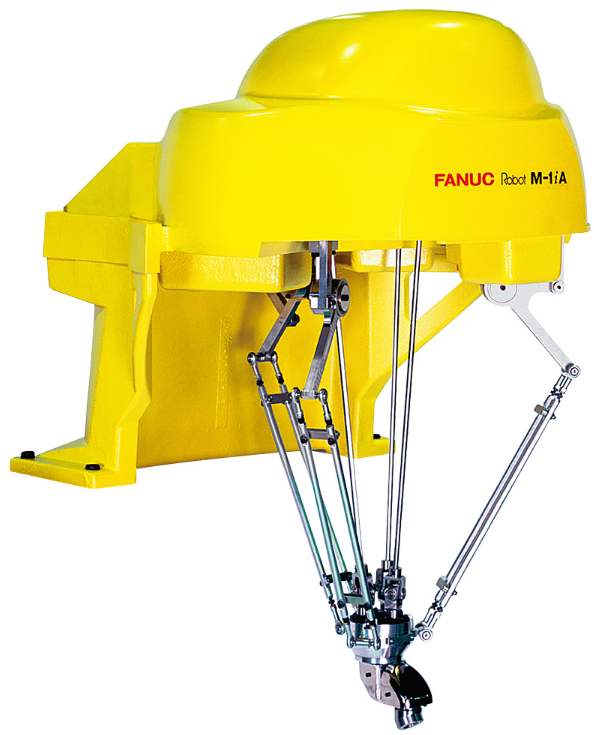
\includegraphics[width=0.25\columnwidth, height=0.2\textwidth]{pic/chap1/FANUC-M-1ia.jpg}
    }
    \subfigure[FlexPicker机器人]{
        \label{fig:robot_example:b}
        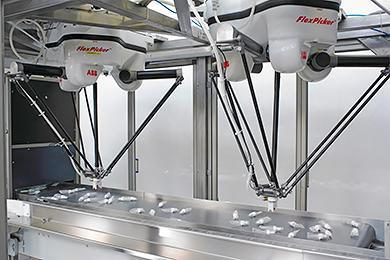
\includegraphics[width=0.25\columnwidth]{pic/chap1/FlexPicker.jpg}
    }
    \subfigure[物流自动分拣机器人]{
        \label{fig:robot_example:c}
        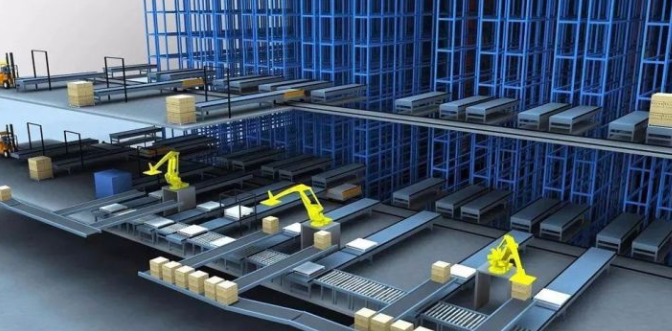
\includegraphics[width=0.5\columnwidth]{pic/chap1/wuliu.jpg}
    }
    \caption{自动分拣机器人实例}
    \label{fig:robot_example}
\end{figure}

目前,国内有多家提供自动分拣解决方案的公司。如深圳辰视智能科技公司,该公司采用传统机器学习方法与深度学习结合的方式定位图像中的目标,引导机械臂对目标采取
相应的操作,以高效低成本的方式为机器人厂家提供机器视觉相关的解决方案。

国外方面,著名的机器人生产厂商如日本的FANUC、EPSON,瑞典的ABB以及德国的KUKA等企业均有自己的自动分拣机器人产品   \cite{HZQ:2016}
。FANUC公司适用于分拣作业的机器人型号为M-1iA型,如图\ref{fig:robot_example}\subref{fig:robot_example:a}
所示。该型号
机器人具有重量轻、结构紧凑的特点,可以安装在各种复杂的环境中。具有快速的响应速度,可以快速调整工件姿态。该机器人配备配套的软件包iRVision内置有各种视觉库,可以完成目标检测
功能,该机器人配备该软件包可实现基于视觉的自动分拣功能。
EPSON公司生产的机器人种类繁多,具有代表性的为S5L型号机器人,其机械结构刚性强、功能强大、运行平稳。基于Vision Guide视觉软件可以实现视觉功能。ABB的FlexPicker机器人则擅长拾取操作,运行
速度快,抓取精度高,非常适用于工件分拣,如图
\ref{fig:robot_example}\subref{fig:robot_example:b}所示。同样,该机器人需要适配Cognex公司生产的配套视觉软件方能实现自动分拣功能。

% %%% 1.2.3 深度学习云平台研究现状
% %%%%%%%%%%%%%%%%%%%%%%%%%%%%%%
% \subsection{深度学习云平台研究现状}
深度学习云平台方面,随着深度学习的高速发展,人工智能逐渐深入到我们的生活当中,而深度学习的高计算资源需求意味着深度学习的高准入门槛,因此,为了满足广大
开发者的深度学习计算需求,一批深度学习云计算平台应运而生。

国内的代表是云计算龙头:阿里云  \cite{aliyun}。
其界面如图\ref{fig:cloud_platform}\subref{fig:cloud_platform:a}所示,
阿里云主要为国内中小企业提供云服务。具体来说,就是将阿里巨量的服务器资源开放出来,
以出租的方式租赁给企业。租赁服务主要包括存储、数据库、企业应用、开发者API等。
其中深度学习服务主要以API的形式对外开放。如果用户需要自行进行深度学习计算,则
需要自行申请带有好计算资源的服务器,通过远程连接到服务器,通过服务器上自带的深度学习框架,自行编写代码进行训练。

\begin{figure}[h]
    \centering
    \subfigure[阿里云界面]{
        \label{fig:cloud_platform:a}
        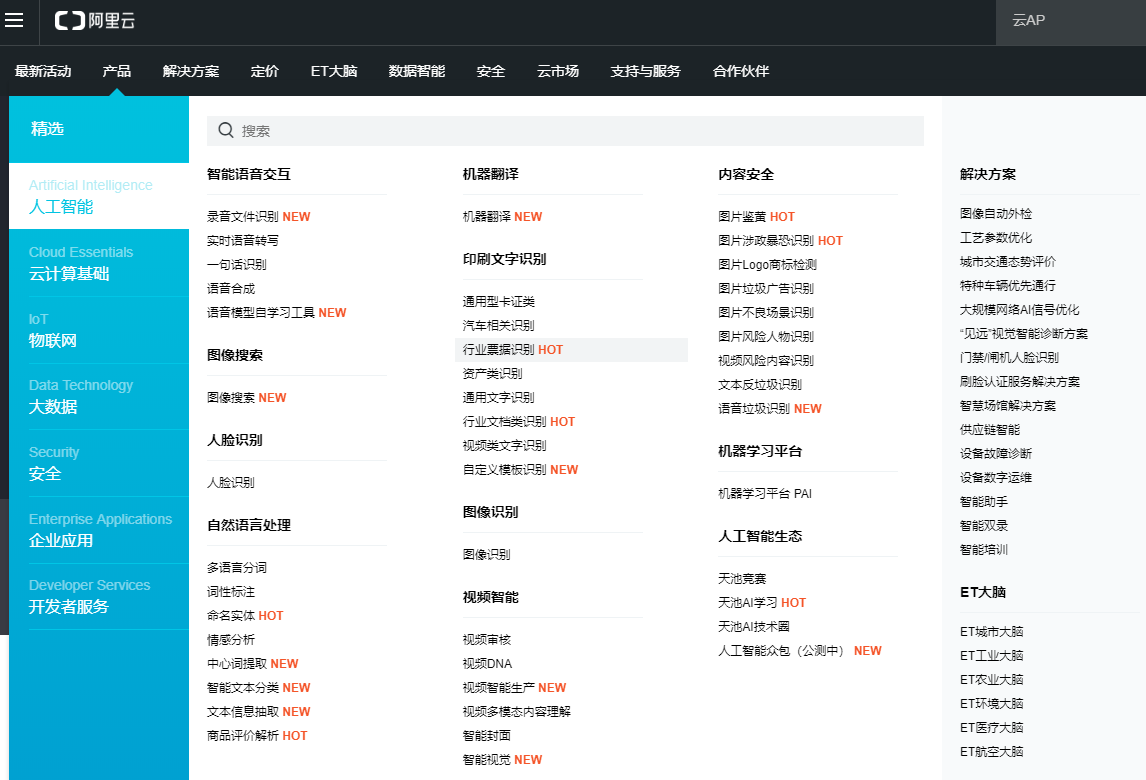
\includegraphics[width=0.4\columnwidth]{pic/chap1/aliyun.jpg}
    }
    \subfigure[谷歌云界面]{
        \label{fig:cloud_platform:b}
        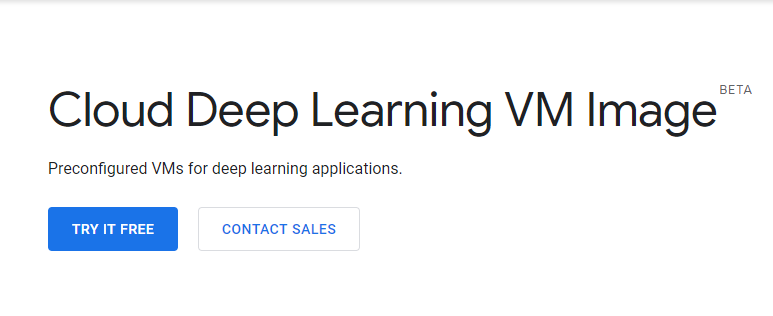
\includegraphics[width=0.4\columnwidth]{pic/chap1/googleyun.jpg}
    }
    \subfigure[亚马逊云界面]{
        \label{fig:cloud_platform:c}
        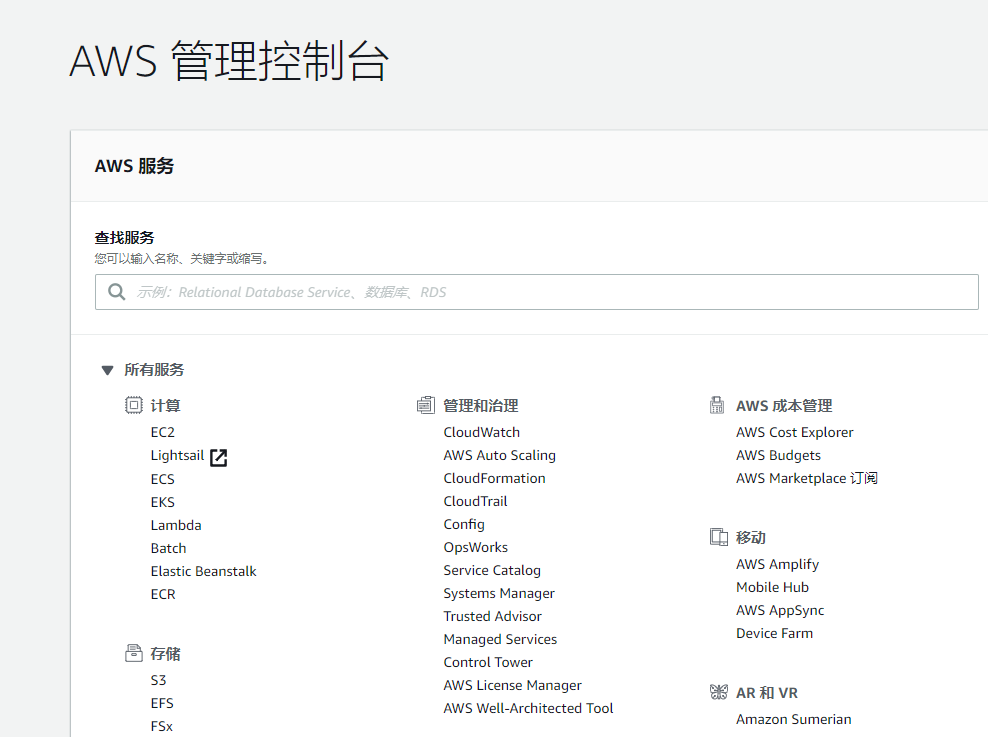
\includegraphics[width=0.4\columnwidth]{pic/chap1/AWSyun.jpg}
    }
    \subfigure[英伟达云界面]{
        \label{fig:cloud_platform:d}
        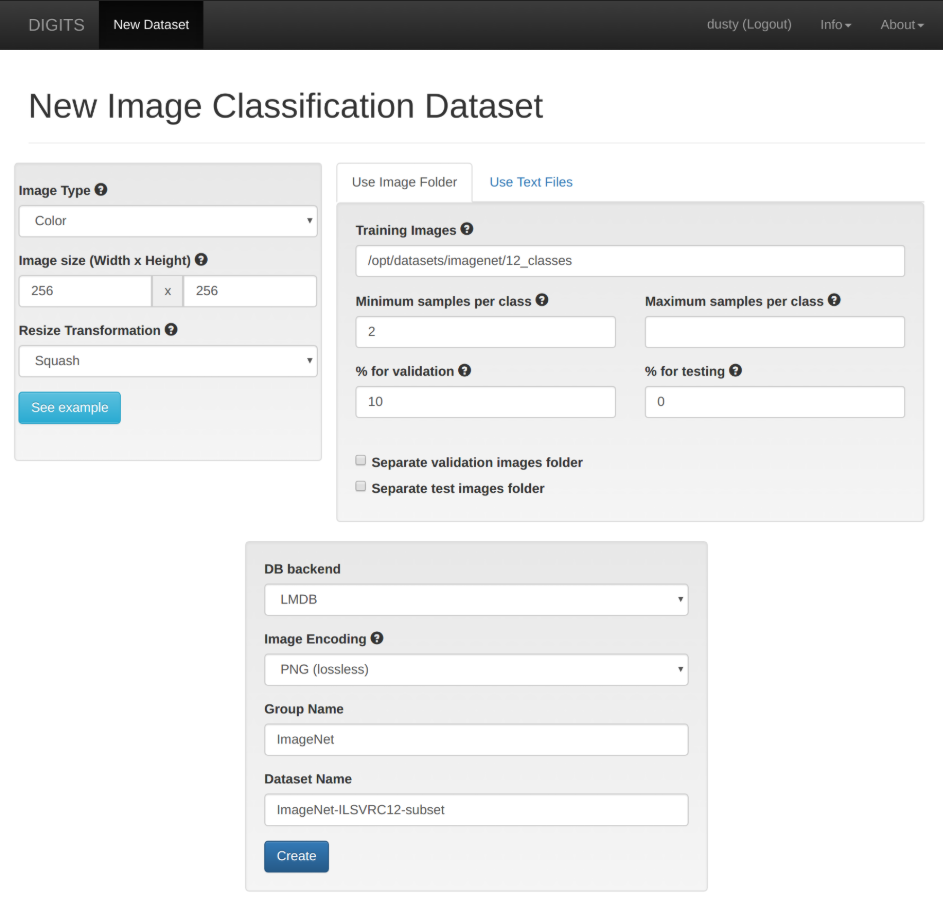
\includegraphics[width=0.4\columnwidth, height=0.3\columnwidth]{pic/chap1/nvidiayun.jpg}
    }
    \caption{国内外云平台实例}
    \label{fig:cloud_platform}
\end{figure}


国外云计算起步较早,如美国的谷歌、亚马逊、英伟达等公司均提供优秀的云服务。其中亚马逊云  \cite{AWSyun}占据了美国市场最大的份额。
亚马逊云界面如图\ref{fig:cloud_platform}\subref{fig:cloud_platform:c}所示。亚马逊云为客户提供功能十分丰富的云服务,其中,深度学习相关资源的提供方式和
阿里云类似。值得一提的是英伟达云(Nvidia GPU Cloud, NGC)    \cite{NVIDIAyun},其界面如图\ref{fig:cloud_platform}\subref{fig:cloud_platform:d},
NGC主要提供深度学习计算服务,并且与阿里云和亚马逊云只提供计算资源不同,NGC将常用的深度学习算法训练过程进行了封装,
通过网页端以选择框和文本框的形式供用户自定义深度学习训练参数配置。同时提供了常用的深度学习数据集供用户使用。用户只需要选择配置和数据集
即可训练自己的深度学习模型,大大降低了深度学习的计算和知识门槛。

综上可知,国内外云计算平台的深度学习服务主要通过API的方式提供,深度学习定制化模型一般只面向具备开发能力的开发者。而我国国内制造业从业者普遍缺乏云计算平台的使用能力
及深度学习知识,即使能够使用云计算提供的高计算资源,也很难去定制自身需要的深度学习模型。因此,针对国内制造业从业者缺乏深度学习知识而制造业又需要深度学习模型落地的具体
情况,开发一款面向制造业的封装良好且易于上手的云平台十分必要。


%%% 1.3 论文研究内容与架构
%%%%%%%%%%%%%%%%%%%%%%%%%%%%%%
\section{论文研究内容与架构}
\subsection{论文研究内容}
自动分拣系统主要由图像采集模块、图像处理模块和机器人模块构成,其中图像处理模块的核心为目标检测算法。传统的自动分拣系统,其主要采取传统的目标检测算法,针对
特定的检测工件,人工构造特征,进行模板匹配工件位置,然后使用这些特征作为分类器的输入再进行分类。总而言之,传统的分拣系统,其采取的目标检测算法需要根据不同
的工件人为构造特征,一旦工件发生变化,需要重新提取特征。这样的系统可移植性较差。随着深度学习的快速发展,基于神经网络的端到端的训练方式逐步改造着视觉方面的各类
算法。神经网络可以在训练过程中自动提取底层和高层特征,能够很好的表征图像特征,无需人为提取和构造特征,且效果也优于传统算法。由于神经网络的特征提取特性,
当工件类别发生变化时,无需耗费过多人力即可完成模型的移植,因此,基于深度学习的目标检测算法具有很好的可移植性。此外,基于国内制造业从业者缺乏深度学习知识和
技能的现状,业内急需一款面向制造业的低门槛深度学习云计算平台。出于以上几点,本论文设计并实验了一个基于深度学习目标检测算法的机械臂分拣系统,并开发了一个用于
定制深度学习目标检测模型的云平台。

本论文一共分为两部分。一是机械臂分拣系统的设计与实验;二是用于定制深度学习目标检测模型的云计算平台。

其中,基于深度学习的机械臂分拣系统需要实现如下功能或模块:
\begin{enumerate}
    \item{图像获取模块,实时获取图像信息,并以一定的通信方式将图片实时传递给图像处理模块。}
    \item{图像处理模块,接收图像获取模块传递来的图像信息,通过训练好的目标检测模型预测该图像中工件的位置及类别,并以一定的通信方式传递给机械臂模块。}
    \item{机械臂执行模块,包括机械臂控制模块和机械臂;接收当前图像中的工件位置和类别信息,将其转化为相应的控制指令,控制机械臂将工件抓起,并放到该工件类别相对应的位置。}
\end{enumerate}

定制深度学习目标检测模型的云计算平台需要实现以下功能:
\begin{enumerate}
    \item{Web端方面,提供文件上传功能,用于接收用户自行标注的数据集,以定制化目标检测模型。}
    \item{同样是Web端,以选择框或文本框的形式给出用户可自定义的超参数选项,方便用户定制化自己需要的模型特性。}
    \item{服务器端,接收Web端发送的各项参数,并根据参数执行相应的shell脚本,调用GPU训练深度学习目标检测模型,并且能够将训练过程中的各项参数实时同步到Web端,方便用户
    可视化模型的训练过程。}
\end{enumerate}

基于深度学习的目标检测模型虽然具有效果好、可移植性强等诸多优点,但其所需计算资源较大,难以在普通的嵌入式平台或台式机上运行,而使用GPU服务器进行实时计算会让整个系统显得
笨重,因此,如何在嵌入式平台进行深度学习模型的预测运算是一个难点。其次,图像采集模块、图像处理模块、机械臂控制模块需要高效的通信机制,以便以高FPS完成采集、处理、执行的流程。
云平台方面,则需要探究Web前端和服务器端的通信机制,及服务器端拿到配置信息后,如何调用GPU去训练深度学习模型。

针对以上问题,本论文针对以下方面进行了深入研究:
\begin{enumerate}
    \item{基于深度学习的目标检测模型的训练。首先搭建图像采集模块,并对所要检测的工件进行图像采集。针对这些图像,使用特定的图像标注工具进行标注。选取Yolov3作为目标检测模型,
    选取其开源框架Darknet进行训练,训练使用两块GTX 1080Ti显卡。并对其训练过程中的各项参数如Loss、IOU等值进行可视化分析。}
    \item{机械臂控制模块的设计实现。由于相机与机械臂所在空间的零点不一致,因此系统在使用之前需要进行标定。将机械臂和相机的坐标统一化。之后分析如何根据相机中工件的位置信息
    计算出机械臂下工件的位置信息,然后研究机械臂的控制方法,控制机械臂执行相应的动作。}
    \item{机器人通信机制研究。使用机器人操作系统(Robot Operation System,ROS)实现图像采集模块、图像处理模块、机械臂控制模块的高效通信。并研究如何将Yolov3模型封装为ROS节点,
    加入整个系统通信网络。}
    \item{云平台结构设计与实现。包括Web前端页面的设计与实现,文件上传功能的实现,使用JavaScript获取前端组件信息,并封装为JSON数据发送给服务端。服务端则需要接收并解析JSON配置数据,并编写相应的Linux
     shell脚本去训练定制化的深度学习模型,并将模型训练过程中的信息实时同步到Web前端。}
\end{enumerate}

\subsection{论文架构}
\begin{figure}
    \centering
    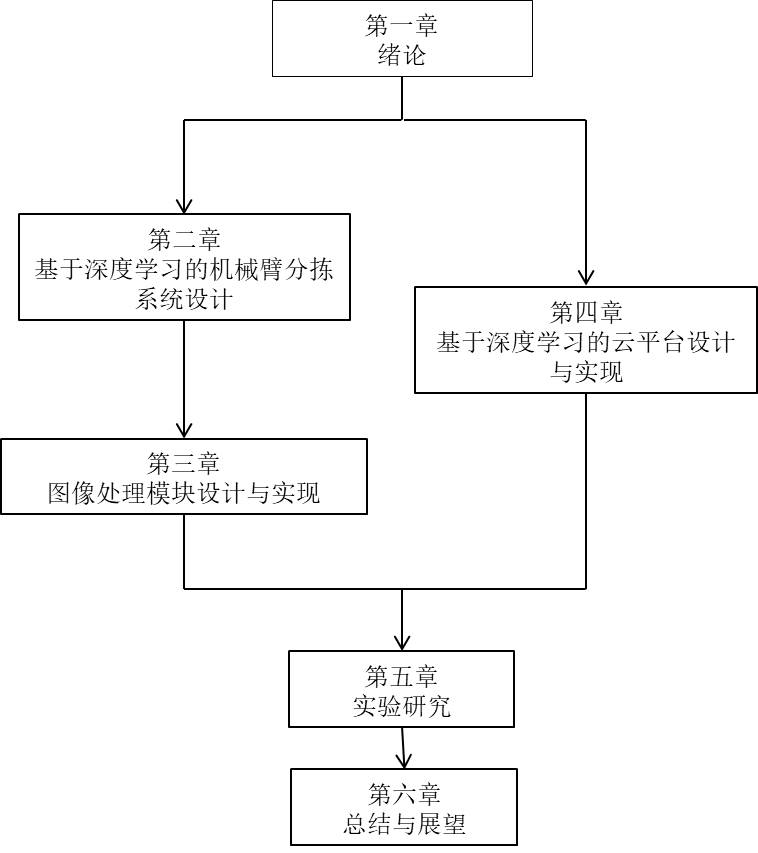
\includegraphics[scale=0.8]{pic/chap1/paper_construct.jpg}
    \caption{论文章节架构}
    \label{fig:paper_construct}
\end{figure}
针对课题的研究内容,本论文各个章节的主要内容安排如下:

第1章,首先阐述了本论文的研究背景和研究意义;然后介绍了目标检测算法、基于视觉的自动分拣系统和深度学习云平台的国内外研究现状;最后给出了本论文的主要研究内容和论文架构。

第2章,主要从整体上阐述了本课题中基于深度学习的机械臂分拣系统的设计方案;并介绍了系统的硬件选型及依据,阐述了系统所使用的通信方案;之后根据本系统的具体条件,选择合适的
深度学习目标检测算法;最后介绍了如何进行相机标定和机械臂控制。

第3章,重点介绍图像处理模块。首先介绍了系统中使用的图像处理算法理论;然后介绍如何使用图像采集模块获取数据集并进行标注;最后是深度学习目标检测模型的训练、评估和部署。

第4章,首先介绍深度学习云平台的整体设计方案和通信方法,并进行了云平台的用户需求分析;之后分别介绍了云平台服务器端和Web端的实现方案。

第5章,分别就本论文的两大部分进行实验。第一部分对所选取的模型配置进行了实验,验证了YOLOv3-tiny模型配置针对本任务的优越性,并对自动分拣系统的延时和准确率进行了实验。第二部分则对深度学习
云平台服务端和Web端进行了稳定性测试实验。

第6章,对本论文所做的工作进行了总结,并对未来可作的改进工作进行了探讨。

论文的章节架构图如图    \ref{fig:paper_construct} 所示。

\section{本章小结}
本章首先阐述了论文的研究背景和研究意义;然后介绍了目标检测算法、基于视觉的自动分拣系统和深度学习云平台的国内外研究现状;最后给出了本论文的主要研究内容和论文架构。